\documentclass[twoside]{book}

% Packages required by doxygen
\usepackage{calc}
\usepackage{doxygen}
\usepackage{graphicx}
\usepackage[utf8]{inputenc}
\usepackage{makeidx}
\usepackage{multicol}
\usepackage{multirow}
\usepackage{textcomp}
\usepackage[table]{xcolor}

% Font selection
\usepackage[T1]{fontenc}
\usepackage{mathptmx}
\usepackage[scaled=.90]{helvet}
\usepackage{courier}
\usepackage{amssymb}
\usepackage{sectsty}
\renewcommand{\familydefault}{\sfdefault}
\allsectionsfont{%
  \fontseries{bc}\selectfont%
  \color{darkgray}%
}
\renewcommand{\DoxyLabelFont}{%
  \fontseries{bc}\selectfont%
  \color{darkgray}%
}

% Page & text layout
\usepackage{geometry}
\geometry{%
  a4paper,%
  top=2.5cm,%
  bottom=2.5cm,%
  left=2.5cm,%
  right=2.5cm%
}
\tolerance=750
\hfuzz=15pt
\hbadness=750
\setlength{\emergencystretch}{15pt}
\setlength{\parindent}{0cm}
\setlength{\parskip}{0.2cm}
\makeatletter
\renewcommand{\paragraph}{%
  \@startsection{paragraph}{4}{0ex}{-1.0ex}{1.0ex}{%
    \normalfont\normalsize\bfseries\SS@parafont%
  }%
}
\renewcommand{\subparagraph}{%
  \@startsection{subparagraph}{5}{0ex}{-1.0ex}{1.0ex}{%
    \normalfont\normalsize\bfseries\SS@subparafont%
  }%
}
\makeatother

% Headers & footers
\usepackage{fancyhdr}
\pagestyle{fancyplain}
\fancyhead[LE]{\fancyplain{}{\bfseries\thepage}}
\fancyhead[CE]{\fancyplain{}{}}
\fancyhead[RE]{\fancyplain{}{\bfseries\leftmark}}
\fancyhead[LO]{\fancyplain{}{\bfseries\rightmark}}
\fancyhead[CO]{\fancyplain{}{}}
\fancyhead[RO]{\fancyplain{}{\bfseries\thepage}}
\fancyfoot[LE]{\fancyplain{}{}}
\fancyfoot[CE]{\fancyplain{}{}}
\fancyfoot[RE]{\fancyplain{}{\bfseries\scriptsize Generated on Fri Feb 14 2014 11\-:39\-:56 for My Project by Doxygen }}
\fancyfoot[LO]{\fancyplain{}{\bfseries\scriptsize Generated on Fri Feb 14 2014 11\-:39\-:56 for My Project by Doxygen }}
\fancyfoot[CO]{\fancyplain{}{}}
\fancyfoot[RO]{\fancyplain{}{}}
\renewcommand{\footrulewidth}{0.4pt}
\renewcommand{\chaptermark}[1]{%
  \markboth{#1}{}%
}
\renewcommand{\sectionmark}[1]{%
  \markright{\thesection\ #1}%
}

% Indices & bibliography
\usepackage{natbib}
\usepackage[titles]{tocloft}
\setcounter{tocdepth}{3}
\setcounter{secnumdepth}{5}
\makeindex

% Hyperlinks (required, but should be loaded last)
\usepackage{ifpdf}
\ifpdf
  \usepackage[pdftex,pagebackref=true]{hyperref}
\else
  \usepackage[ps2pdf,pagebackref=true]{hyperref}
\fi
\hypersetup{%
  colorlinks=true,%
  linkcolor=blue,%
  citecolor=blue,%
  unicode%
}

% Custom commands
\newcommand{\clearemptydoublepage}{%
  \newpage{\pagestyle{empty}\cleardoublepage}%
}


%===== C O N T E N T S =====

\begin{document}

% Titlepage & ToC
\hypersetup{pageanchor=false}
\pagenumbering{roman}
\begin{titlepage}
\vspace*{7cm}
\begin{center}%
{\Large My Project }\\
\vspace*{1cm}
{\large Generated by Doxygen 1.8.6}\\
\vspace*{0.5cm}
{\small Fri Feb 14 2014 11:39:56}\\
\end{center}
\end{titlepage}
\clearemptydoublepage
\tableofcontents
\clearemptydoublepage
\pagenumbering{arabic}
\hypersetup{pageanchor=true}

%--- Begin generated contents ---
\chapter{Hierarchical Index}
\section{Class Hierarchy}
This inheritance list is sorted roughly, but not completely, alphabetically\-:\begin{DoxyCompactList}
\item \contentsline{section}{Animation}{\pageref{class_animation}}{}
\item \contentsline{section}{dynamic\-Body}{\pageref{structdynamic_body}}{}
\item \contentsline{section}{Entity}{\pageref{class_entity}}{}
\begin{DoxyCompactList}
\item \contentsline{section}{Monster}{\pageref{class_monster}}{}
\begin{DoxyCompactList}
\item \contentsline{section}{Ramachandra}{\pageref{class_ramachandra}}{}
\end{DoxyCompactList}
\end{DoxyCompactList}
\item \contentsline{section}{Entity\-Container}{\pageref{class_entity_container}}{}
\item \contentsline{section}{Map}{\pageref{class_map}}{}
\item Neural\-Network\begin{DoxyCompactList}
\item \contentsline{section}{Monster}{\pageref{class_monster}}{}
\end{DoxyCompactList}
\item Non\-Copyable\begin{DoxyCompactList}
\item \contentsline{section}{Simulation}{\pageref{class_simulation}}{}
\end{DoxyCompactList}
\item Population\begin{DoxyCompactList}
\item \contentsline{section}{Ramachandra\-Population}{\pageref{class_ramachandra_population}}{}
\end{DoxyCompactList}
\item Sprite\begin{DoxyCompactList}
\item \contentsline{section}{Button}{\pageref{class_button}}{}
\begin{DoxyCompactList}
\item \contentsline{section}{Adjust\-Middle\-Button}{\pageref{class_adjust_middle_button}}{}
\end{DoxyCompactList}
\end{DoxyCompactList}
\item \contentsline{section}{State}{\pageref{class_state}}{}
\begin{DoxyCompactList}
\item \contentsline{section}{Main\-Menu}{\pageref{class_main_menu}}{}
\item \contentsline{section}{Splash}{\pageref{class_splash}}{}
\end{DoxyCompactList}
\item \contentsline{section}{static\-Body}{\pageref{structstatic_body}}{}
\item \contentsline{section}{static\-Rectangle\-Body}{\pageref{structstatic_rectangle_body}}{}
\item \contentsline{section}{Texture\-Holder}{\pageref{class_texture_holder}}{}
\end{DoxyCompactList}

\chapter{Class Index}
\section{Class List}
Here are the classes, structs, unions and interfaces with brief descriptions\-:\begin{DoxyCompactList}
\item\contentsline{section}{\hyperlink{class_adjust_middle_button}{Adjust\-Middle\-Button} \\*This class adjusts the position of the button from the middle when the screen size changes }{\pageref{class_adjust_middle_button}}{}
\item\contentsline{section}{\hyperlink{class_animation}{Animation} }{\pageref{class_animation}}{}
\item\contentsline{section}{\hyperlink{class_button}{Button} }{\pageref{class_button}}{}
\item\contentsline{section}{\hyperlink{structdynamic_body}{dynamic\-Body} }{\pageref{structdynamic_body}}{}
\item\contentsline{section}{\hyperlink{class_entity}{Entity} }{\pageref{class_entity}}{}
\item\contentsline{section}{\hyperlink{class_entity_container}{Entity\-Container} }{\pageref{class_entity_container}}{}
\item\contentsline{section}{\hyperlink{class_main_menu}{Main\-Menu} }{\pageref{class_main_menu}}{}
\item\contentsline{section}{\hyperlink{class_map}{Map} }{\pageref{class_map}}{}
\item\contentsline{section}{\hyperlink{class_monster}{Monster} }{\pageref{class_monster}}{}
\item\contentsline{section}{\hyperlink{class_ramachandra}{Ramachandra} }{\pageref{class_ramachandra}}{}
\item\contentsline{section}{\hyperlink{class_ramachandra_population}{Ramachandra\-Population} }{\pageref{class_ramachandra_population}}{}
\item\contentsline{section}{\hyperlink{class_simulation}{Simulation} }{\pageref{class_simulation}}{}
\item\contentsline{section}{\hyperlink{class_splash}{Splash} }{\pageref{class_splash}}{}
\item\contentsline{section}{\hyperlink{class_state}{State} }{\pageref{class_state}}{}
\item\contentsline{section}{\hyperlink{structstatic_body}{static\-Body} }{\pageref{structstatic_body}}{}
\item\contentsline{section}{\hyperlink{structstatic_rectangle_body}{static\-Rectangle\-Body} }{\pageref{structstatic_rectangle_body}}{}
\item\contentsline{section}{\hyperlink{class_texture_holder}{Texture\-Holder} }{\pageref{class_texture_holder}}{}
\end{DoxyCompactList}

\chapter{Class Documentation}
\hypertarget{class_adjust_middle_button}{\section{Adjust\-Middle\-Button Class Reference}
\label{class_adjust_middle_button}\index{Adjust\-Middle\-Button@{Adjust\-Middle\-Button}}
}


This class adjusts the position of the button from the middle when the screen size changes.  




{\ttfamily \#include $<$Adjust\-Middle\-Button.\-hpp$>$}

Inheritance diagram for Adjust\-Middle\-Button\-:\begin{figure}[H]
\begin{center}
\leavevmode
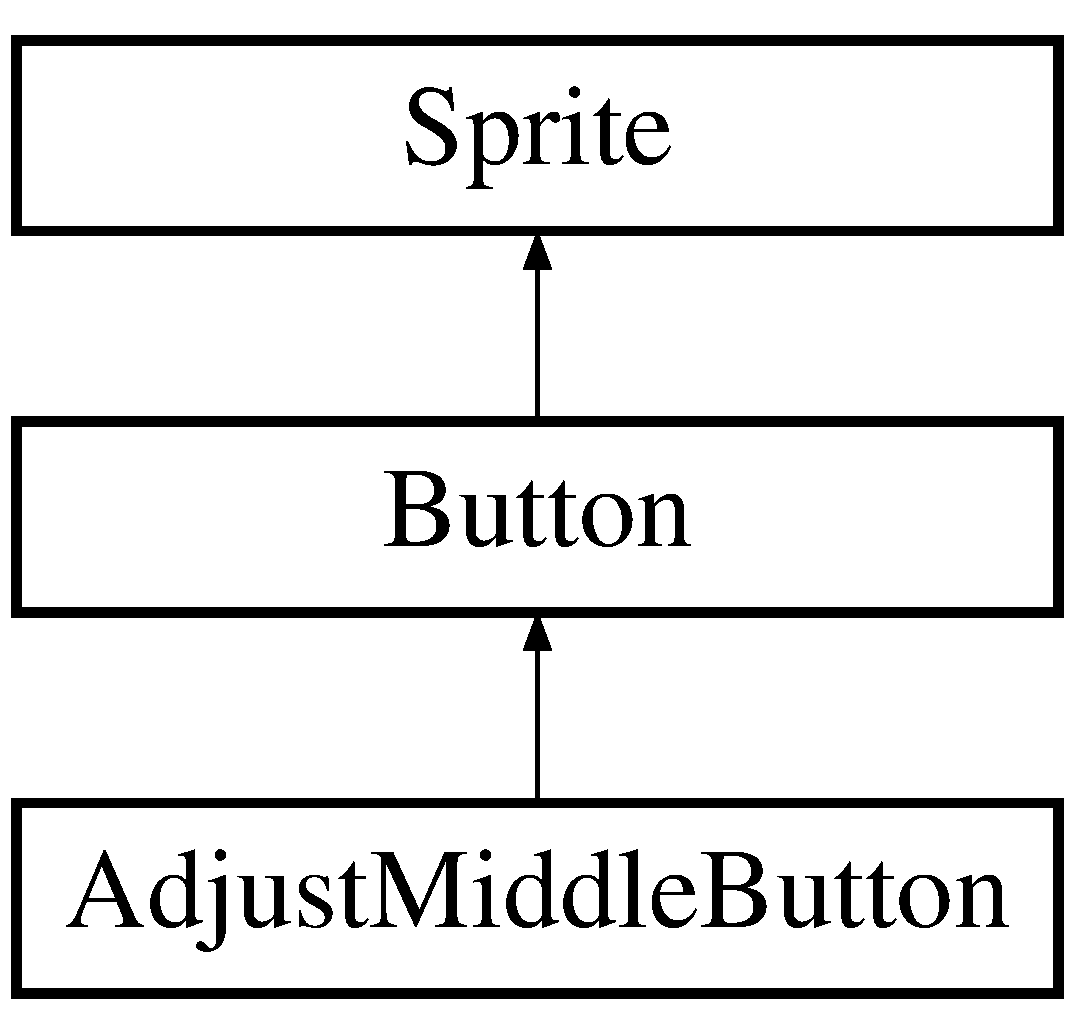
\includegraphics[height=3.000000cm]{class_adjust_middle_button}
\end{center}
\end{figure}
\subsection*{Public Member Functions}
\begin{DoxyCompactItemize}
\item 
\hypertarget{class_adjust_middle_button_a9946c953357138786dbcd91c7c72bfd7}{bool {\bfseries update} (sf\-::\-Render\-Window \&Window)}\label{class_adjust_middle_button_a9946c953357138786dbcd91c7c72bfd7}

\item 
\hypertarget{class_adjust_middle_button_abb760233fcd96e9efed1271e23727891}{{\bfseries Adjust\-Middle\-Button} (const sf\-::\-Texture \&texture)}\label{class_adjust_middle_button_abb760233fcd96e9efed1271e23727891}

\item 
\hypertarget{class_adjust_middle_button_a0d20b68fa8981fdc61811b4a2fa557e1}{\hyperlink{class_adjust_middle_button_a0d20b68fa8981fdc61811b4a2fa557e1}{Adjust\-Middle\-Button} (const sf\-::\-Texture \&texture, sf\-::\-Vector2f \hyperlink{class_adjust_middle_button_a9a89c5d3f24d0fe7e85d5eb1c6d16110}{position})}\label{class_adjust_middle_button_a0d20b68fa8981fdc61811b4a2fa557e1}

\begin{DoxyCompactList}\small\item\em Position is from center. \end{DoxyCompactList}\item 
\hypertarget{class_adjust_middle_button_a1b10b9e9fa40fc575cdb664aacd0cbc0}{\hyperlink{class_adjust_middle_button_a1b10b9e9fa40fc575cdb664aacd0cbc0}{Adjust\-Middle\-Button} (sf\-::\-Vector2f \hyperlink{class_adjust_middle_button_a9a89c5d3f24d0fe7e85d5eb1c6d16110}{position})}\label{class_adjust_middle_button_a1b10b9e9fa40fc575cdb664aacd0cbc0}

\begin{DoxyCompactList}\small\item\em Position is from center. \end{DoxyCompactList}\item 
void \hyperlink{class_adjust_middle_button_a9a89c5d3f24d0fe7e85d5eb1c6d16110}{position} (sf\-::\-Vector2f position)
\item 
\hypertarget{class_adjust_middle_button_aaa0ebf98f00093ec9c9bfe1e0fc92793}{void {\bfseries position} (float x, float y)}\label{class_adjust_middle_button_aaa0ebf98f00093ec9c9bfe1e0fc92793}

\item 
\hypertarget{class_adjust_middle_button_a80d1f7ea96d67dd35d5dd41ef3a82485}{void \hyperlink{class_adjust_middle_button_a80d1f7ea96d67dd35d5dd41ef3a82485}{render} (sf\-::\-Render\-Window \&Window)}\label{class_adjust_middle_button_a80d1f7ea96d67dd35d5dd41ef3a82485}

\begin{DoxyCompactList}\small\item\em render is used instead of draw to allow seemless moving for buttons that need it \end{DoxyCompactList}\end{DoxyCompactItemize}
\subsection*{Public Attributes}
\begin{DoxyCompactItemize}
\item 
\hypertarget{class_adjust_middle_button_a4ceef445de03b2b38073ff73a296def1}{sf\-::\-Vector2f {\bfseries position\-From\-Center}}\label{class_adjust_middle_button_a4ceef445de03b2b38073ff73a296def1}

\end{DoxyCompactItemize}
\subsection*{Additional Inherited Members}


\subsection{Detailed Description}
This class adjusts the position of the button from the middle when the screen size changes. 

\subsection{Member Function Documentation}
\hypertarget{class_adjust_middle_button_a9a89c5d3f24d0fe7e85d5eb1c6d16110}{\index{Adjust\-Middle\-Button@{Adjust\-Middle\-Button}!position@{position}}
\index{position@{position}!AdjustMiddleButton@{Adjust\-Middle\-Button}}
\subsubsection[{position}]{\setlength{\rightskip}{0pt plus 5cm}void Adjust\-Middle\-Button\-::position (
\begin{DoxyParamCaption}
\item[{sf\-::\-Vector2f}]{position}
\end{DoxyParamCaption}
)}}\label{class_adjust_middle_button_a9a89c5d3f24d0fe7e85d5eb1c6d16110}
Position must be according to the center of the screen

It is not set\-Position() because that interferes with access to Transformable. 

The documentation for this class was generated from the following files\-:\begin{DoxyCompactItemize}
\item 
Adjust\-Middle\-Button.\-hpp\item 
Adjust\-Middle\-Button.\-cpp\end{DoxyCompactItemize}

\hypertarget{class_animation}{\section{Animation Class Reference}
\label{class_animation}\index{Animation@{Animation}}
}
\subsection*{Public Member Functions}
\begin{DoxyCompactItemize}
\item 
\hypertarget{class_animation_a7258506ebfa4b6edbb249bb49a0ff036}{{\bfseries Animation} (sf\-::\-Time init\-Sprite\-Time)}\label{class_animation_a7258506ebfa4b6edbb249bb49a0ff036}

\item 
\hypertarget{class_animation_a379fff9002fe0d7ef80854ff5252d3ba}{sf\-::\-Int\-Rect {\bfseries get\-Animation} ()}\label{class_animation_a379fff9002fe0d7ef80854ff5252d3ba}

\item 
\hypertarget{class_animation_a9a3cc9d923251460cddd99800486c717}{void {\bfseries add\-Rectangle} (sf\-::\-Int\-Rect new\-Rect)}\label{class_animation_a9a3cc9d923251460cddd99800486c717}

\item 
\hypertarget{class_animation_a0746fa52ca85e0313398e1c3895a49f3}{bool {\bfseries new\-Sprite} ()}\label{class_animation_a0746fa52ca85e0313398e1c3895a49f3}

\end{DoxyCompactItemize}


The documentation for this class was generated from the following files\-:\begin{DoxyCompactItemize}
\item 
Animation.\-hpp\item 
Animation.\-cpp\end{DoxyCompactItemize}

\hypertarget{class_button}{\section{Button Class Reference}
\label{class_button}\index{Button@{Button}}
}
Inheritance diagram for Button\-:\begin{figure}[H]
\begin{center}
\leavevmode
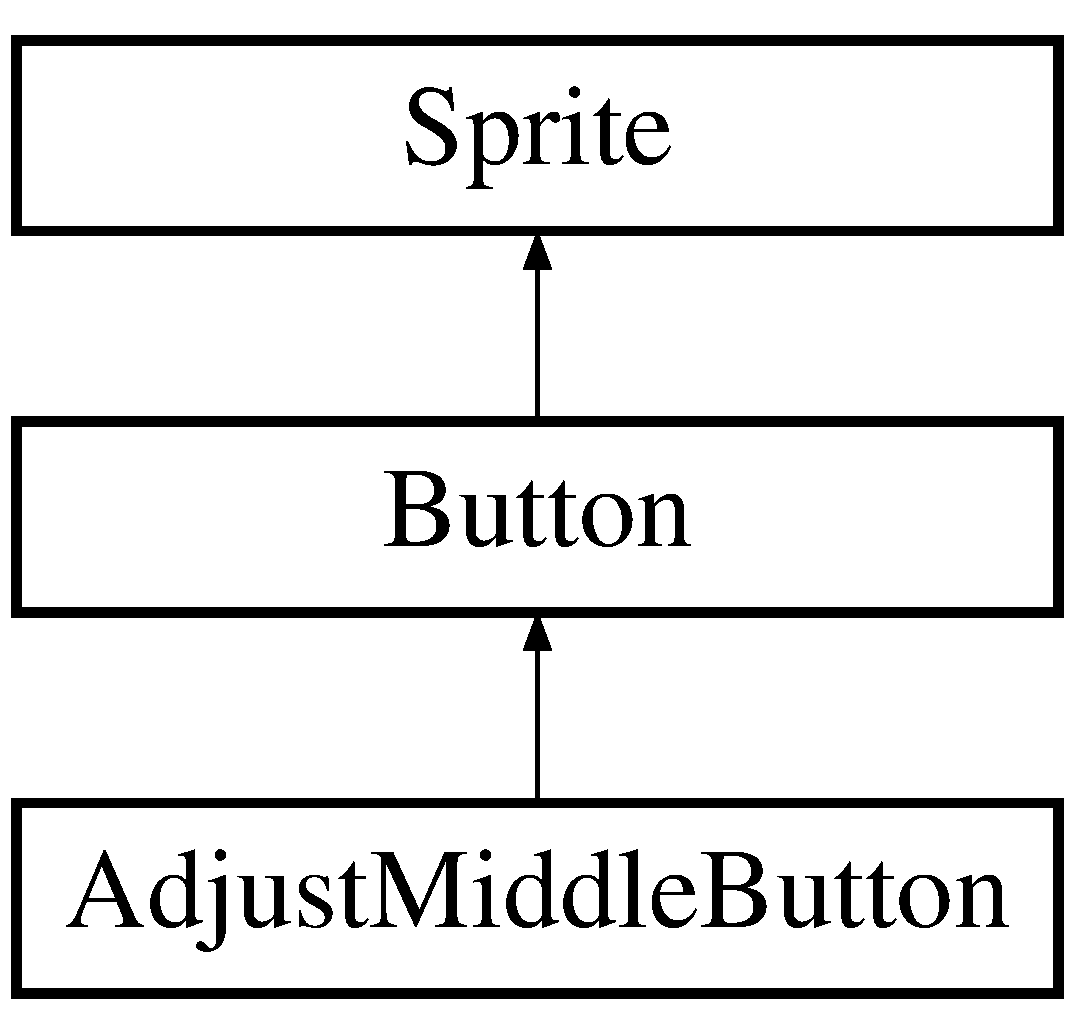
\includegraphics[height=3.000000cm]{class_button}
\end{center}
\end{figure}
\subsection*{Public Member Functions}
\begin{DoxyCompactItemize}
\item 
\hypertarget{class_button_a0ac5ee796c96cada2f46ec53d90b9d64}{bool {\bfseries update} (sf\-::\-Render\-Window \&window)}\label{class_button_a0ac5ee796c96cada2f46ec53d90b9d64}

\item 
\hypertarget{class_button_a740a5437a98746507da2d6d854777f90}{{\bfseries Button} (const sf\-::\-Texture \&texture)}\label{class_button_a740a5437a98746507da2d6d854777f90}

\item 
\hypertarget{class_button_a16e7549156216234a6111b24d6d2bd62}{void \hyperlink{class_button_a16e7549156216234a6111b24d6d2bd62}{render} (sf\-::\-Render\-Window \&Window)}\label{class_button_a16e7549156216234a6111b24d6d2bd62}

\begin{DoxyCompactList}\small\item\em render is used instead of draw to allow seemless moving for buttons that need it \end{DoxyCompactList}\end{DoxyCompactItemize}
\subsection*{Protected Attributes}
\begin{DoxyCompactItemize}
\item 
\hypertarget{class_button_a301a025a5f248413230198380cff086f}{sf\-::\-Clock {\bfseries cooldown\-Counter}}\label{class_button_a301a025a5f248413230198380cff086f}

\item 
\hypertarget{class_button_a00ae9520611d006294a7f53c4796a95e}{const sf\-::\-Time {\bfseries cooldown}}\label{class_button_a00ae9520611d006294a7f53c4796a95e}

\end{DoxyCompactItemize}


The documentation for this class was generated from the following files\-:\begin{DoxyCompactItemize}
\item 
Button.\-hpp\item 
Button.\-cpp\end{DoxyCompactItemize}

\hypertarget{structdynamic_body}{\section{dynamic\-Body Struct Reference}
\label{structdynamic_body}\index{dynamic\-Body@{dynamic\-Body}}
}
\subsection*{Public Attributes}
\begin{DoxyCompactItemize}
\item 
\hypertarget{structdynamic_body_ae8e99ba778d0b451a0fcde9618ccd701}{b2\-Polygon\-Shape {\bfseries dynamic\-Shape}}\label{structdynamic_body_ae8e99ba778d0b451a0fcde9618ccd701}

\item 
\hypertarget{structdynamic_body_a7462e596fac525f60295fd8ad4bf7112}{b2\-Body\-Def {\bfseries body\-Def}}\label{structdynamic_body_a7462e596fac525f60295fd8ad4bf7112}

\item 
\hypertarget{structdynamic_body_a4d3f717a8113be7c019c14fd5e90d181}{b2\-Body $\ast$ {\bfseries body}}\label{structdynamic_body_a4d3f717a8113be7c019c14fd5e90d181}

\item 
\hypertarget{structdynamic_body_ae8cfdf22a1cf26cab93118d0f1ba30bf}{b2\-Fixture\-Def {\bfseries fixture\-Def}}\label{structdynamic_body_ae8cfdf22a1cf26cab93118d0f1ba30bf}

\end{DoxyCompactItemize}


The documentation for this struct was generated from the following file\-:\begin{DoxyCompactItemize}
\item 
Body\-Structs.\-hpp\end{DoxyCompactItemize}

\hypertarget{class_entity}{\section{Entity Class Reference}
\label{class_entity}\index{Entity@{Entity}}
}
Inheritance diagram for Entity\-:\begin{figure}[H]
\begin{center}
\leavevmode
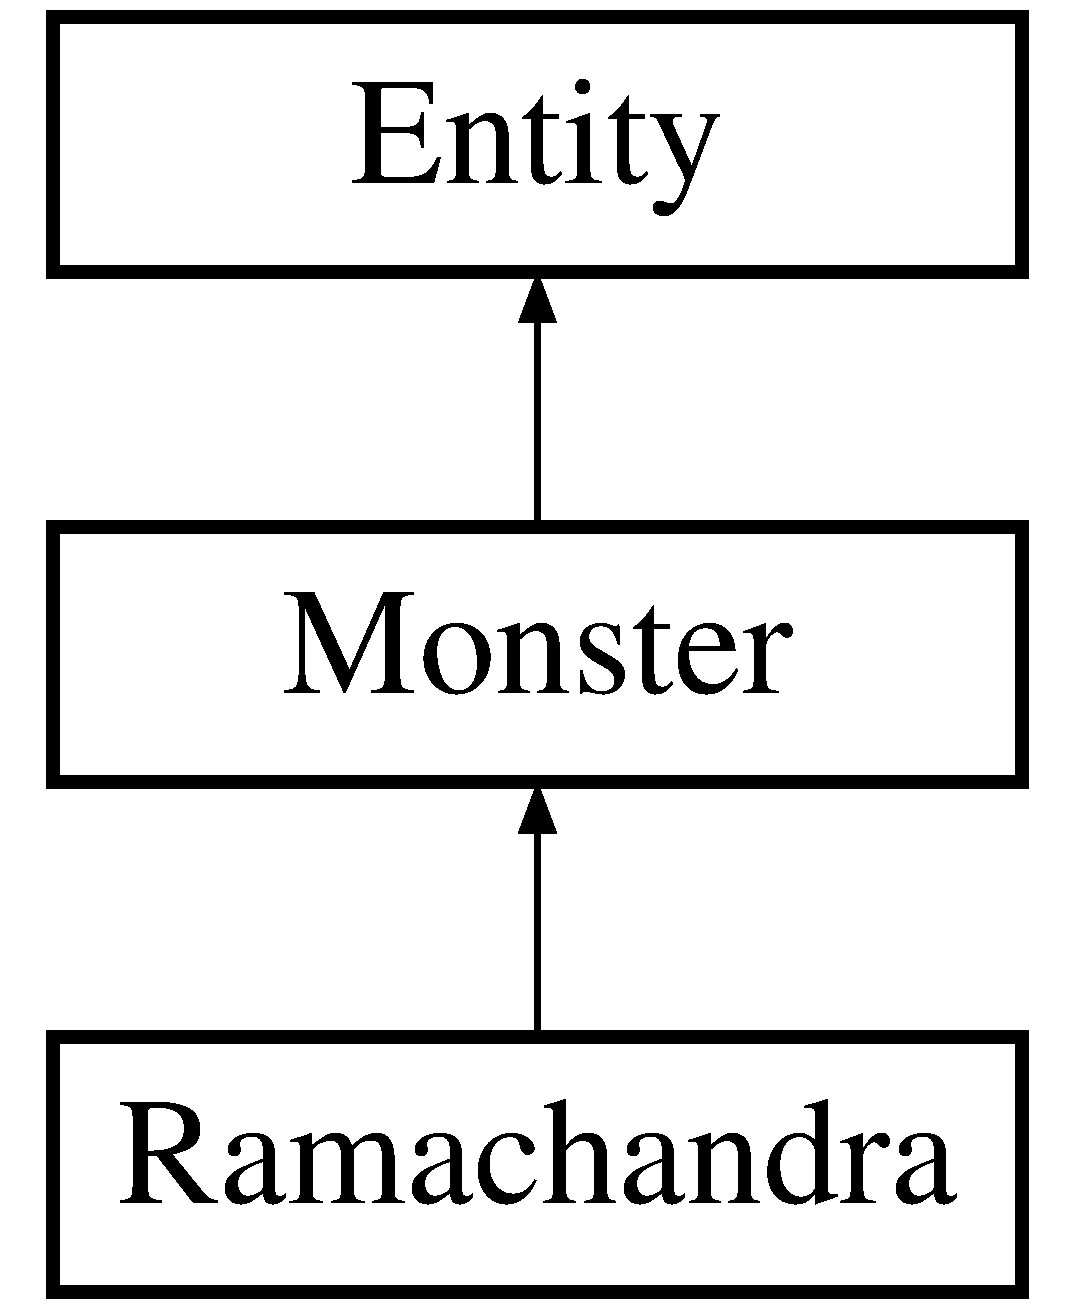
\includegraphics[height=3.000000cm]{class_entity}
\end{center}
\end{figure}
\subsection*{Public Member Functions}
\begin{DoxyCompactItemize}
\item 
\hypertarget{class_entity_a7b3312cce57dd71b479a0d85232c3bcf}{virtual void {\bfseries update} (\hyperlink{class_map}{Map} \&map, sf\-::\-Time \&elapsed\-Time)}\label{class_entity_a7b3312cce57dd71b479a0d85232c3bcf}

\item 
\hypertarget{class_entity_a7ed67f40d2626b3b79667b3c56a27c90}{virtual void {\bfseries render} (sf\-::\-Render\-Window \&Window)}\label{class_entity_a7ed67f40d2626b3b79667b3c56a27c90}

\item 
\hypertarget{class_entity_abc5b6d26c039bf3bf6faa766990768b4}{float {\bfseries get\-X} ()}\label{class_entity_abc5b6d26c039bf3bf6faa766990768b4}

\item 
\hypertarget{class_entity_ab6dd7b404c13754202acfe3d2c65c77b}{float {\bfseries get\-Y} ()}\label{class_entity_ab6dd7b404c13754202acfe3d2c65c77b}

\item 
\hypertarget{class_entity_abe6071cb041670ae7211b5e91c00a84a}{float {\bfseries get\-Width} ()}\label{class_entity_abe6071cb041670ae7211b5e91c00a84a}

\item 
\hypertarget{class_entity_af461ab9c4738878b3160806d92f91e3a}{float {\bfseries get\-Height} ()}\label{class_entity_af461ab9c4738878b3160806d92f91e3a}

\item 
\hypertarget{class_entity_a3c60d3c0561843490e93bde1f4566900}{virtual int {\bfseries get\-I\-D} ()}\label{class_entity_a3c60d3c0561843490e93bde1f4566900}

\end{DoxyCompactItemize}
\subsection*{Protected Attributes}
\begin{DoxyCompactItemize}
\item 
\hypertarget{class_entity_a48ef4ab143b8d0211877c9f6be42e824}{sf\-::\-Sprite {\bfseries sprite}}\label{class_entity_a48ef4ab143b8d0211877c9f6be42e824}

\item 
\hypertarget{class_entity_a1eb77bbf42f194fe03ecdeec3cbe8ad0}{sf\-::\-Texture $\ast$ {\bfseries texture}}\label{class_entity_a1eb77bbf42f194fe03ecdeec3cbe8ad0}

\end{DoxyCompactItemize}


The documentation for this class was generated from the following files\-:\begin{DoxyCompactItemize}
\item 
Entity.\-hpp\item 
Entity.\-cpp\end{DoxyCompactItemize}

\hypertarget{class_entity_container}{\section{Entity\-Container Class Reference}
\label{class_entity_container}\index{Entity\-Container@{Entity\-Container}}
}
\subsection*{Public Member Functions}
\begin{DoxyCompactItemize}
\item 
\hypertarget{class_entity_container_ac0c475afef35afacc68222858c7c1235}{virtual void {\bfseries update} (\hyperlink{class_map}{Map} \&map, sf\-::\-Time \&elapsed\-Time)}\label{class_entity_container_ac0c475afef35afacc68222858c7c1235}

\item 
\hypertarget{class_entity_container_af531a5ba2b41416fdb96c879b6d8a322}{virtual void {\bfseries render} (sf\-::\-Render\-Window \&Window)}\label{class_entity_container_af531a5ba2b41416fdb96c879b6d8a322}

\item 
\hypertarget{class_entity_container_a12f72f7801d0a84977a8909952ffbf62}{\hyperlink{class_entity}{Entity} $\ast$ {\bfseries get\-Entity} (int index)}\label{class_entity_container_a12f72f7801d0a84977a8909952ffbf62}

\item 
\hypertarget{class_entity_container_adfe05295a0f40712bd07f0fb1f7c03d4}{void {\bfseries add\-Entity} (\hyperlink{class_entity}{Entity} $\ast$new\-Entity)}\label{class_entity_container_adfe05295a0f40712bd07f0fb1f7c03d4}

\item 
\hypertarget{class_entity_container_a39817a5176ff360fcf935b95eeef7f73}{virtual void {\bfseries empty} ()}\label{class_entity_container_a39817a5176ff360fcf935b95eeef7f73}

\item 
\hypertarget{class_entity_container_a8f950aea4e2c12ef425fff9c4b718247}{virtual int {\bfseries amount} ()}\label{class_entity_container_a8f950aea4e2c12ef425fff9c4b718247}

\end{DoxyCompactItemize}
\subsection*{Protected Attributes}
\begin{DoxyCompactItemize}
\item 
\hypertarget{class_entity_container_aa68925e602b9f5836a65ec47e1f85921}{std\-::vector$<$ \hyperlink{class_entity}{Entity} $\ast$ $>$ {\bfseries entities}}\label{class_entity_container_aa68925e602b9f5836a65ec47e1f85921}

\end{DoxyCompactItemize}


The documentation for this class was generated from the following files\-:\begin{DoxyCompactItemize}
\item 
Entity\-Container.\-hpp\item 
Entity\-Container.\-cpp\end{DoxyCompactItemize}

\hypertarget{class_main_menu}{\section{Main\-Menu Class Reference}
\label{class_main_menu}\index{Main\-Menu@{Main\-Menu}}
}
Inheritance diagram for Main\-Menu\-:\begin{figure}[H]
\begin{center}
\leavevmode
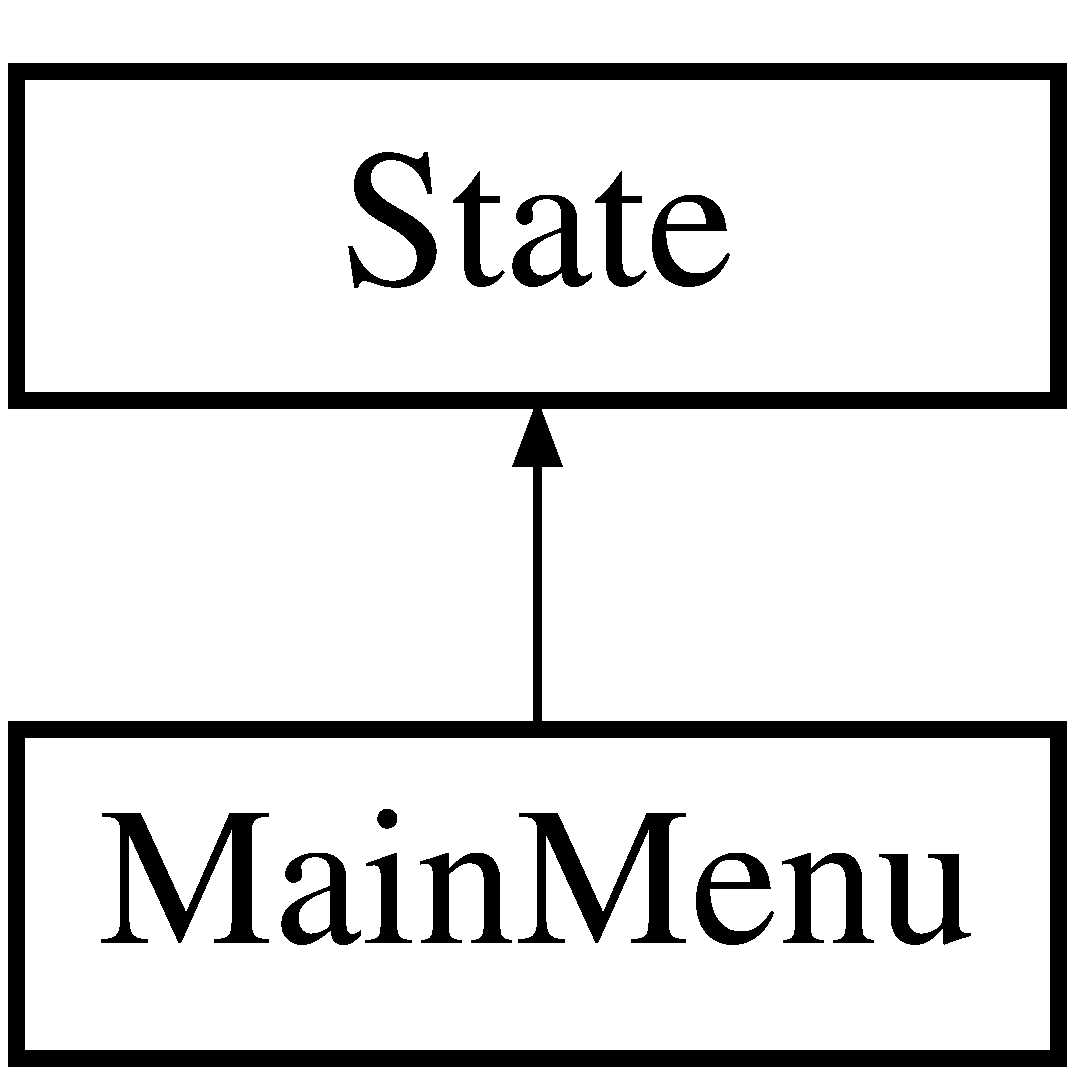
\includegraphics[height=2.000000cm]{class_main_menu}
\end{center}
\end{figure}
\subsection*{Public Member Functions}
\begin{DoxyCompactItemize}
\item 
\hypertarget{class_main_menu_a9b9354471b9401a72a9b0c259331f6c0}{\hyperlink{class_main_menu_a9b9354471b9401a72a9b0c259331f6c0}{Main\-Menu} (sf\-::\-Render\-Window \&Window, \hyperlink{class_texture_holder}{Texture\-Holder} \&textures\-Holder)}\label{class_main_menu_a9b9354471b9401a72a9b0c259331f6c0}

\begin{DoxyCompactList}\small\item\em N\-O\-T\-E\-: inherited. \end{DoxyCompactList}\end{DoxyCompactItemize}


The documentation for this class was generated from the following files\-:\begin{DoxyCompactItemize}
\item 
Main\-Menu.\-hpp\item 
Main\-Menu.\-cpp\end{DoxyCompactItemize}

\hypertarget{class_map}{\section{Map Class Reference}
\label{class_map}\index{Map@{Map}}
}
\subsection*{Public Member Functions}
\begin{DoxyCompactItemize}
\item 
\hypertarget{class_map_a3e104473a3b574971e843a025e0e05bd}{{\bfseries Map} (int arg\-Map\-Size, b2\-World $\ast$world)}\label{class_map_a3e104473a3b574971e843a025e0e05bd}

\item 
\hypertarget{class_map_a58b5deaadf39f7bada29153f2f5395d9}{void {\bfseries render} (sf\-::\-Render\-Window \&Window)}\label{class_map_a58b5deaadf39f7bada29153f2f5395d9}

\item 
\hypertarget{class_map_a839effe30ba3687f91bd5d559ea065dd}{int {\bfseries get\-Map\-Size} ()}\label{class_map_a839effe30ba3687f91bd5d559ea065dd}

\item 
\hypertarget{class_map_a52759e6f15c7d73e9073c0811439adfb}{void \hyperlink{class_map_a52759e6f15c7d73e9073c0811439adfb}{create\-Map\-Bodies} (b2\-World \&world)}\label{class_map_a52759e6f15c7d73e9073c0811439adfb}

\begin{DoxyCompactList}\small\item\em Do not call in the constructor of map! \end{DoxyCompactList}\end{DoxyCompactItemize}


The documentation for this class was generated from the following files\-:\begin{DoxyCompactItemize}
\item 
Map.\-hpp\item 
Map.\-cpp\end{DoxyCompactItemize}

\hypertarget{class_monster}{\section{Monster Class Reference}
\label{class_monster}\index{Monster@{Monster}}
}
Inheritance diagram for Monster\-:\begin{figure}[H]
\begin{center}
\leavevmode
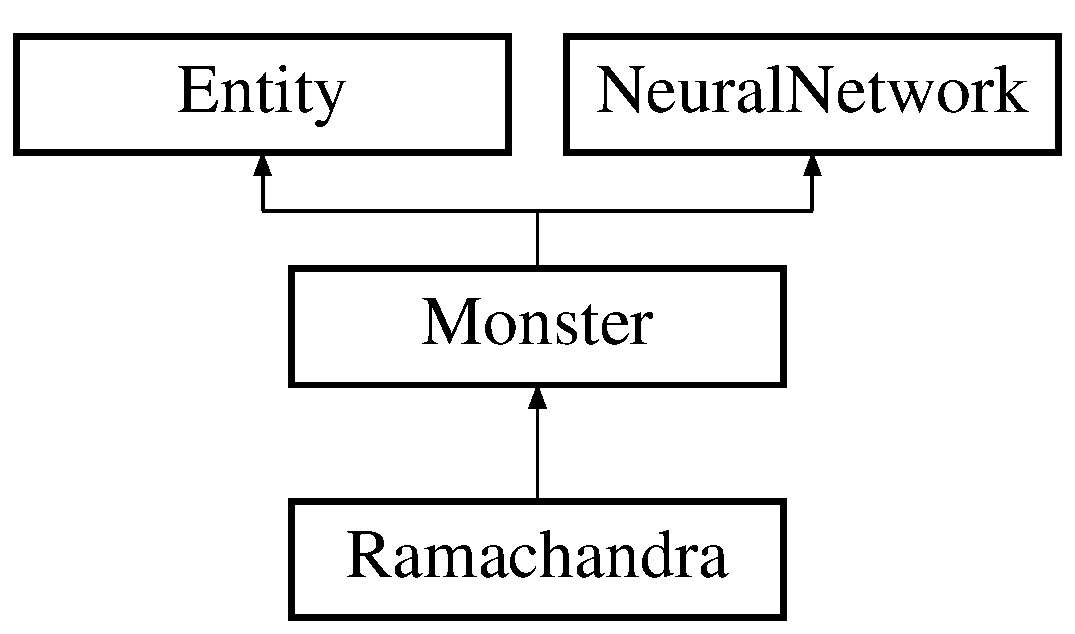
\includegraphics[height=3.000000cm]{class_monster}
\end{center}
\end{figure}
\subsection*{Public Member Functions}
\begin{DoxyCompactItemize}
\item 
\hypertarget{class_monster_aeff591902eae79493bd713883f1356c5}{virtual void {\bfseries update} (b2\-World \&world, sf\-::\-Time \&elapsed\-Time)}\label{class_monster_aeff591902eae79493bd713883f1356c5}

\item 
\hypertarget{class_monster_a4d194dc47ad8d4a87cc2f58df7fdc624}{virtual void {\bfseries render} (sf\-::\-Render\-Window \&Window)}\label{class_monster_a4d194dc47ad8d4a87cc2f58df7fdc624}

\item 
\hypertarget{class_monster_ac93ae314a09c74e90206adbd59b5547d}{unsigned long long {\bfseries get\-Fitness} ()}\label{class_monster_ac93ae314a09c74e90206adbd59b5547d}

\item 
\hypertarget{class_monster_ae915f10d3a2cfd6172b8f5d96a209bdd}{bool {\bfseries get\-Dead} ()}\label{class_monster_ae915f10d3a2cfd6172b8f5d96a209bdd}

\item 
\hypertarget{class_monster_af1ded6e0a1365439cc7261072bfc42e6}{virtual void {\bfseries resurrect} (b2\-World \&world, float x\-Coord, float y\-Coord)}\label{class_monster_af1ded6e0a1365439cc7261072bfc42e6}

\item 
\hypertarget{class_monster_a96b2fd8a63a477aeb39ea5e97c1b9535}{virtual int {\bfseries get\-I\-D} ()}\label{class_monster_a96b2fd8a63a477aeb39ea5e97c1b9535}

\end{DoxyCompactItemize}
\subsection*{Protected Member Functions}
\begin{DoxyCompactItemize}
\item 
\hypertarget{class_monster_a88596b981f071c8deec021966bcd2644}{std\-::vector$<$ double $>$ {\bfseries get\-Inputs} ()}\label{class_monster_a88596b981f071c8deec021966bcd2644}

\item 
\hypertarget{class_monster_a8d9f9ec59c821c786318cba7118330de}{virtual void {\bfseries set\-Textures} (\hyperlink{class_texture_holder}{Texture\-Holder} \&texture\-Holder)}\label{class_monster_a8d9f9ec59c821c786318cba7118330de}

\item 
\hypertarget{class_monster_adad8414146dd91707a451f5d153d12fb}{virtual void {\bfseries animate} ()}\label{class_monster_adad8414146dd91707a451f5d153d12fb}

\item 
\hypertarget{class_monster_a932cd4f0fc8044cc873e5550b3cf10c3}{virtual void {\bfseries set\-Animations} ()}\label{class_monster_a932cd4f0fc8044cc873e5550b3cf10c3}

\item 
\hypertarget{class_monster_a1bfc08ef5073ae736ffad4de8844bbf4}{{\bfseries Monster} (int x\-Tile, int y\-Tile, \hyperlink{class_map}{Map} \&map, \hyperlink{class_texture_holder}{Texture\-Holder} \&texture\-Holder, b2\-World \&world)}\label{class_monster_a1bfc08ef5073ae736ffad4de8844bbf4}

\item 
\hypertarget{class_monster_a802abc56224cd726540cecc3e6221cf1}{virtual void {\bfseries create\-Body} (b2\-World \&world, float x\-Coord, float y\-Coord)}\label{class_monster_a802abc56224cd726540cecc3e6221cf1}

\end{DoxyCompactItemize}
\subsection*{Protected Attributes}
\begin{DoxyCompactItemize}
\item 
\hypertarget{class_monster_a06d47971b7f78a6a3867f15ff6d14688}{unsigned long long {\bfseries fitness\-Value}}\label{class_monster_a06d47971b7f78a6a3867f15ff6d14688}

\item 
\hypertarget{class_monster_a7dcdcbd51514aa5f77cfb317ad8f54ad}{int {\bfseries hunger}}\label{class_monster_a7dcdcbd51514aa5f77cfb317ad8f54ad}

\item 
\hypertarget{class_monster_af37d637fecf6ec0792fd008d7b3f32f9}{bool {\bfseries dead\-Flag}}\label{class_monster_af37d637fecf6ec0792fd008d7b3f32f9}

\item 
\hypertarget{class_monster_a6ca9674730dc6997e7e5fb6f5b019686}{\hyperlink{structdynamic_body}{dynamic\-Body} {\bfseries body}}\label{class_monster_a6ca9674730dc6997e7e5fb6f5b019686}

\end{DoxyCompactItemize}


The documentation for this class was generated from the following files\-:\begin{DoxyCompactItemize}
\item 
Monster.\-hpp\item 
Monster.\-cpp\end{DoxyCompactItemize}

\hypertarget{class_ramachandra}{\section{Ramachandra Class Reference}
\label{class_ramachandra}\index{Ramachandra@{Ramachandra}}
}
Inheritance diagram for Ramachandra\-:\begin{figure}[H]
\begin{center}
\leavevmode
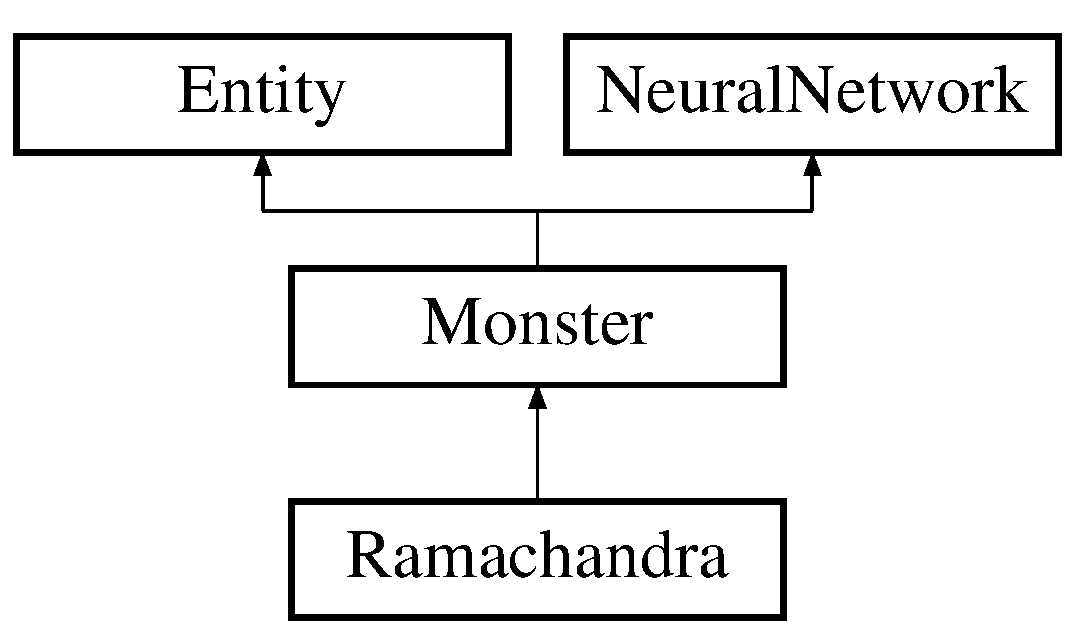
\includegraphics[height=3.000000cm]{class_ramachandra}
\end{center}
\end{figure}
\subsection*{Public Member Functions}
\begin{DoxyCompactItemize}
\item 
\hypertarget{class_ramachandra_a5c1789c5f2e0a5236fcc82a7f20833d2}{{\bfseries Ramachandra} (int x\-Coord, int y\-Coord, \hyperlink{class_map}{Map} \&map, \hyperlink{class_texture_holder}{Texture\-Holder} \&texture\-Holder, b2\-World \&world)}\label{class_ramachandra_a5c1789c5f2e0a5236fcc82a7f20833d2}

\item 
\hypertarget{class_ramachandra_a2f544c9a55f310ec8ccc86c65552f449}{virtual void {\bfseries update} (b2\-World \&world, sf\-::\-Time \&elapsed\-Time)}\label{class_ramachandra_a2f544c9a55f310ec8ccc86c65552f449}

\item 
\hypertarget{class_ramachandra_ace94fd3bbaefa2a068de5b38c9960bf4}{virtual void {\bfseries render} (sf\-::\-Render\-Window \&Window)}\label{class_ramachandra_ace94fd3bbaefa2a068de5b38c9960bf4}

\item 
\hypertarget{class_ramachandra_a31d975d2e07814e3166793cd9cb87c2e}{virtual void {\bfseries resurrect} (b2\-World \&world, float x\-Coord, float y\-Coord)}\label{class_ramachandra_a31d975d2e07814e3166793cd9cb87c2e}

\item 
\hypertarget{class_ramachandra_a09e324917322b4b80a74b098b1a1ae1b}{virtual int {\bfseries get\-I\-D} ()}\label{class_ramachandra_a09e324917322b4b80a74b098b1a1ae1b}

\end{DoxyCompactItemize}
\subsection*{Additional Inherited Members}


The documentation for this class was generated from the following files\-:\begin{DoxyCompactItemize}
\item 
Ramachandra.\-hpp\item 
Ramachandra.\-cpp\end{DoxyCompactItemize}

\hypertarget{class_ramachandra_population}{\section{Ramachandra\-Population Class Reference}
\label{class_ramachandra_population}\index{Ramachandra\-Population@{Ramachandra\-Population}}
}
Inheritance diagram for Ramachandra\-Population\-:\begin{figure}[H]
\begin{center}
\leavevmode
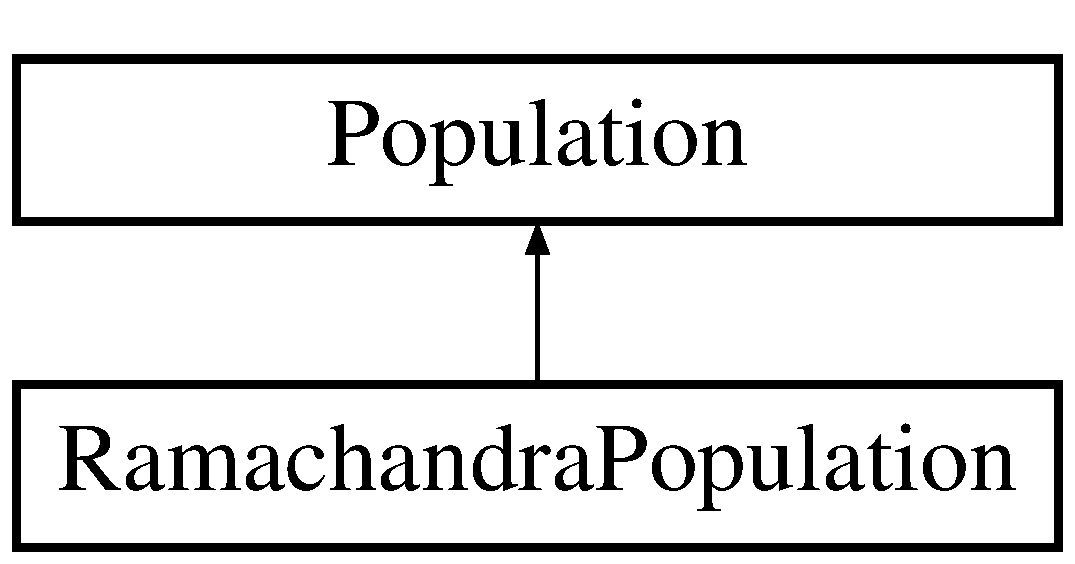
\includegraphics[height=2.000000cm]{class_ramachandra_population}
\end{center}
\end{figure}
\subsection*{Public Member Functions}
\begin{DoxyCompactItemize}
\item 
\hypertarget{class_ramachandra_population_a62dd339d535b148ca6dde79c757a6660}{void {\bfseries initiate} (int initial\-Population, \hyperlink{class_map}{Map} \&map, \hyperlink{class_texture_holder}{Texture\-Holder} \&textures, b2\-World \&world)}\label{class_ramachandra_population_a62dd339d535b148ca6dde79c757a6660}

\end{DoxyCompactItemize}


The documentation for this class was generated from the following files\-:\begin{DoxyCompactItemize}
\item 
Ramachandra\-Population.\-hpp\item 
Ramachandra\-Population.\-cpp\end{DoxyCompactItemize}

\hypertarget{class_simulation}{\section{Simulation Class Reference}
\label{class_simulation}\index{Simulation@{Simulation}}
}
Inheritance diagram for Simulation\-:\begin{figure}[H]
\begin{center}
\leavevmode
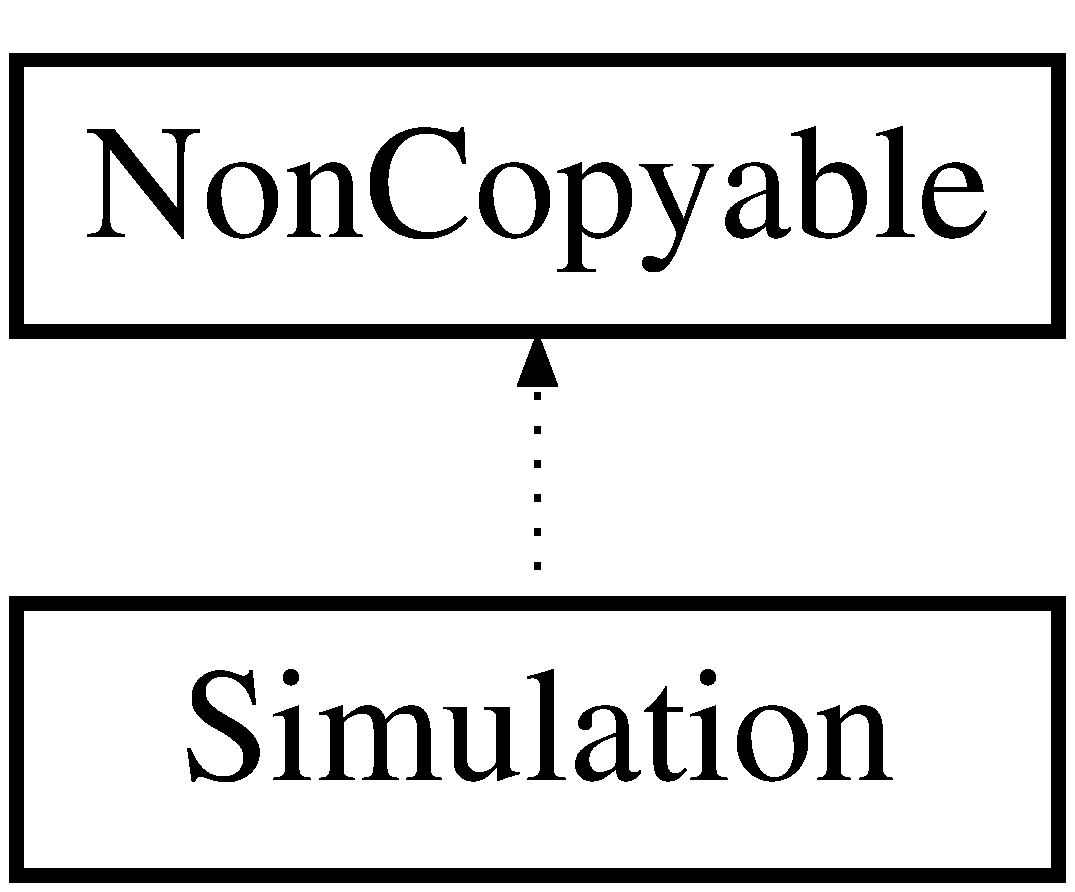
\includegraphics[height=2.000000cm]{class_simulation}
\end{center}
\end{figure}
\subsection*{Public Member Functions}
\begin{DoxyCompactItemize}
\item 
\hypertarget{class_simulation_a18efa4acf8da95ff406d747f69a85542}{{\bfseries Simulation} (int arg\-Map\-Size, std\-::string level, sf\-::\-Render\-Window \&window, \hyperlink{class_texture_holder}{Texture\-Holder} \&texture\-Holder)}\label{class_simulation_a18efa4acf8da95ff406d747f69a85542}

\item 
\hypertarget{class_simulation_ae5c367f87c0b5dc9740bc6d00e44e72c}{void {\bfseries run} ()}\label{class_simulation_ae5c367f87c0b5dc9740bc6d00e44e72c}

\end{DoxyCompactItemize}


The documentation for this class was generated from the following files\-:\begin{DoxyCompactItemize}
\item 
Simulation.\-hpp\item 
Simulation.\-cpp\end{DoxyCompactItemize}

\hypertarget{class_splash}{\section{Splash Class Reference}
\label{class_splash}\index{Splash@{Splash}}
}
Inheritance diagram for Splash\-:\begin{figure}[H]
\begin{center}
\leavevmode
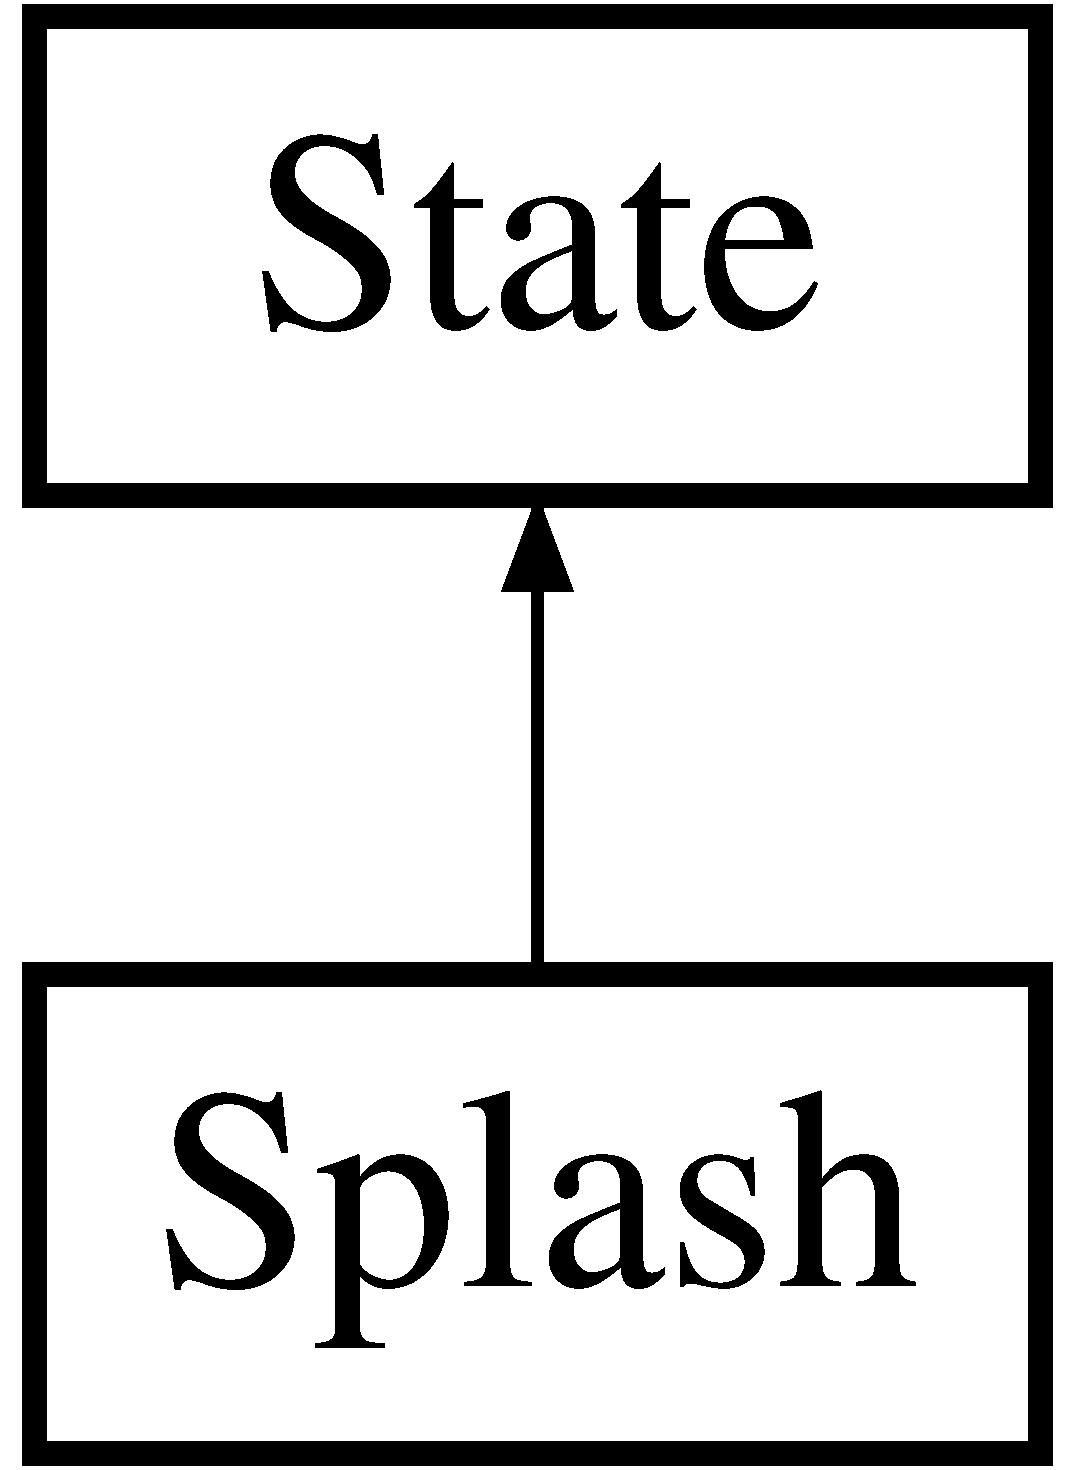
\includegraphics[height=2.000000cm]{class_splash}
\end{center}
\end{figure}
\subsection*{Public Member Functions}
\begin{DoxyCompactItemize}
\item 
\hypertarget{class_splash_a2241fe067b1fa921d37918e5cb240d59}{\hyperlink{class_splash_a2241fe067b1fa921d37918e5cb240d59}{Splash} (sf\-::\-Render\-Window \&Window, int frames)}\label{class_splash_a2241fe067b1fa921d37918e5cb240d59}

\begin{DoxyCompactList}\small\item\em N\-O\-T\-E\-: inherited. \end{DoxyCompactList}\end{DoxyCompactItemize}


The documentation for this class was generated from the following files\-:\begin{DoxyCompactItemize}
\item 
Splash.\-hpp\item 
Splash.\-cpp\end{DoxyCompactItemize}

\hypertarget{class_state}{\section{State Class Reference}
\label{class_state}\index{State@{State}}
}
Inheritance diagram for State\-:\begin{figure}[H]
\begin{center}
\leavevmode
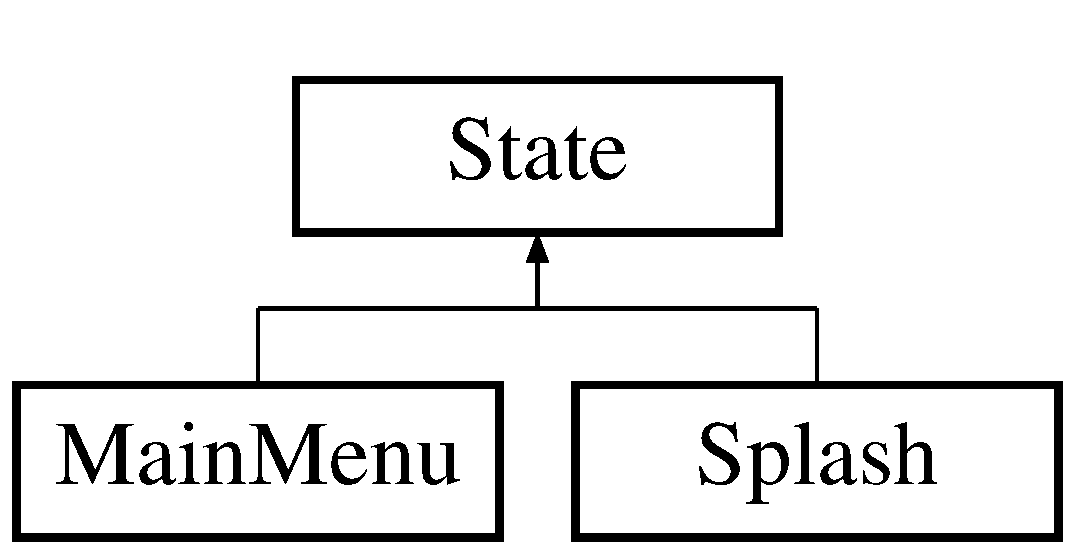
\includegraphics[height=2.000000cm]{class_state}
\end{center}
\end{figure}
\subsection*{Public Member Functions}
\begin{DoxyCompactItemize}
\item 
\hypertarget{class_state_a0084b959e9435631dee76073044434e6}{{\bfseries State} (sf\-::\-Render\-Window \&Window, int frames)}\label{class_state_a0084b959e9435631dee76073044434e6}

\end{DoxyCompactItemize}


The documentation for this class was generated from the following files\-:\begin{DoxyCompactItemize}
\item 
State.\-hpp\item 
State.\-cpp\end{DoxyCompactItemize}

\hypertarget{structstatic_body}{\section{static\-Body Struct Reference}
\label{structstatic_body}\index{static\-Body@{static\-Body}}
}
\subsection*{Public Attributes}
\begin{DoxyCompactItemize}
\item 
\hypertarget{structstatic_body_a1315c6cd5f3473621aa470170286cbeb}{b2\-Body\-Def {\bfseries body\-Def}}\label{structstatic_body_a1315c6cd5f3473621aa470170286cbeb}

\item 
\hypertarget{structstatic_body_a6e1b92e9d231e6be48f53683cf43620a}{b2\-Body $\ast$ {\bfseries body}}\label{structstatic_body_a6e1b92e9d231e6be48f53683cf43620a}

\item 
\hypertarget{structstatic_body_a3d0943215d4baf0c7c83b2ab5ea67d3f}{b2\-Polygon\-Shape {\bfseries shape}}\label{structstatic_body_a3d0943215d4baf0c7c83b2ab5ea67d3f}

\end{DoxyCompactItemize}


The documentation for this struct was generated from the following file\-:\begin{DoxyCompactItemize}
\item 
Body\-Structs.\-hpp\end{DoxyCompactItemize}

\hypertarget{structstatic_rectangle_body}{\section{static\-Rectangle\-Body Struct Reference}
\label{structstatic_rectangle_body}\index{static\-Rectangle\-Body@{static\-Rectangle\-Body}}
}
\subsection*{Public Attributes}
\begin{DoxyCompactItemize}
\item 
\hypertarget{structstatic_rectangle_body_a48e87e9482f138f97786ad3017b0b801}{b2\-Body\-Def {\bfseries body\-Def}}\label{structstatic_rectangle_body_a48e87e9482f138f97786ad3017b0b801}

\item 
\hypertarget{structstatic_rectangle_body_ab7a72fbd213aa720bf795fbeaf94fdbc}{b2\-Body $\ast$ {\bfseries body}}\label{structstatic_rectangle_body_ab7a72fbd213aa720bf795fbeaf94fdbc}

\item 
\hypertarget{structstatic_rectangle_body_ac786c29d811bd890e9aec2a9ca856d76}{b2\-Polygon\-Shape {\bfseries shape}}\label{structstatic_rectangle_body_ac786c29d811bd890e9aec2a9ca856d76}

\item 
\hypertarget{structstatic_rectangle_body_a4fad1dd8686ca44c36086662b54fb1fe}{sf\-::\-Rectangle\-Shape {\bfseries rectangle}}\label{structstatic_rectangle_body_a4fad1dd8686ca44c36086662b54fb1fe}

\end{DoxyCompactItemize}


The documentation for this struct was generated from the following file\-:\begin{DoxyCompactItemize}
\item 
Body\-Structs.\-hpp\end{DoxyCompactItemize}

\hypertarget{class_texture_holder}{\section{Texture\-Holder Class Reference}
\label{class_texture_holder}\index{Texture\-Holder@{Texture\-Holder}}
}
\subsection*{Public Attributes}
\begin{DoxyCompactItemize}
\item 
\hypertarget{class_texture_holder_a8e5c63064c00c3b693dd78ec3b636fec}{sf\-::\-Texture {\bfseries ramachandra}}\label{class_texture_holder_a8e5c63064c00c3b693dd78ec3b636fec}

\item 
\hypertarget{class_texture_holder_aa7bf75dcef805fbd8e979ac35fd3002e}{sf\-::\-Texture {\bfseries t\-Main\-Menu}}\label{class_texture_holder_aa7bf75dcef805fbd8e979ac35fd3002e}

\item 
\hypertarget{class_texture_holder_a5c758224eb37c10e052b4a88adc7d774}{sf\-::\-Texture {\bfseries t\-Play\-Button}}\label{class_texture_holder_a5c758224eb37c10e052b4a88adc7d774}

\end{DoxyCompactItemize}


The documentation for this class was generated from the following files\-:\begin{DoxyCompactItemize}
\item 
Texture\-Holder.\-hpp\item 
Texture\-Holder.\-cpp\end{DoxyCompactItemize}

%--- End generated contents ---

% Index
\newpage
\phantomsection
\addcontentsline{toc}{chapter}{Index}
\printindex

\end{document}
